\chapter{La atm\'osfera}
 
 La capa gaseosa que rodea la Tierra se le conoce como atm\'osfera, los planetas peque\~nos poseen menos atmósfera por que tiene menos masa. En la Tierra la  mayor parte de la masa se acumula en los primeros 11 \kilo\metre\,  de altura (aproximadamente el 95\% del aire se ubica en la primera capa). Los gases son atra\'{\i}dos por la gravedad y se mantienen debido a \'esta, si la gravedad no es suficiente la atm\'osfera es barrida por el viento solar, como ocurre en otros planetas.


 \section{Estructura de la Atm\'osfera}
  Las capas de la atm\'osfera son las siguientes y se pueden ver en la figura~\ref{capasATM} :


\textbf{Exosfera}  se encuentra ubicada a 500\kilo\metre\, posee \'atomos y mol\'eculas no unidas por la gravedad.

\textbf{ Term\'osfera }Se extiende aproximadamente entre 400 y 500~\kilo\metre, con una densidad molecular significativamente menor que en la superficie terrestre, oscilando entre $10^6$ y $10^{14}$ moléculas/\centi\cubic\metre. La temperatura en esta capa varía entre 1,000 y 2,000~\kelvin.  
 \index{atmosfera@atmósfera!estructura}
En la termósfera predominan los átomos de \ce{O2} y \ce{N2}, y su química está principalmente gobernada por la radiación ultravioleta con longitudes de onda $\lambda \leq 150$~\nano\metre. En particular, las transiciones $\alpha$ y $\beta$ ocurren a 121.6~\nano\metre   y 102.6~\nano\metre, respectivamente. Además, esta región es donde se encuentran los rayos X que interactúan con la atmósfera superior.
 \begin{wrapfigure}[27]{r}{35mm}
\centering
%\begin{figure}[htbp]
%\begin{center}
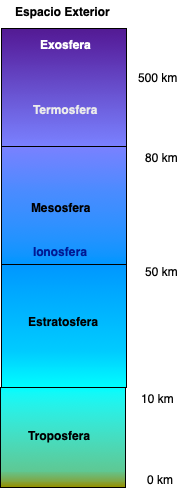
\includegraphics[width=0.30\textwidth]{atmosfera_capas.png}
 %\vspace{-110pt}
\caption{Capas de la atm\'osfera}
\label{capasATM}
%\end{center}
%\end{figure}
\end{wrapfigure}

\textbf{Mesósfera}: Se extiende aproximadamente entre 50 y 100~\kilo\metre~($\pm10$). La concentración de moléculas en esta capa varía entre $10^{13}$ y $10^{16}$ moléculas/centímetro cúbico. La temperatura oscila en un rango de 130 -- 250~\kelvin.  

La química de la mesosfera está dominada por la interacción con la radiación ultravioleta de longitud de onda $\lambda = 250$~\nano\metre. En esta región se encuentran moléculas simples como \ce{O2}, \ce{N2}, \ce{CO2}, \ce{H2O} y \ce{O3}, además de radicales como \ce{OH} y \ce{HO2}, así como iones como \ce{O2-} y \ce{NO2-}.
 

 \textbf{Ionosfera} Sobre 60 \kilo\metre. Se encuentran electrones libres cuya concentraci\'on puede alcanzar $10^6$molec/cc. En esta capa se da la propagaci\'on de las ondas de radio.
 
 \textbf{Estratosfera} Como su nombre lo indica esta en capas de $10-17 \kilo\metre$ hasta $50\kilo\metre$. El mezclado vertical toma a\~nos. La qu\'{\i}mica es dirigida por luz ultravioleta, visible con longitudes de onda mayores a los 175\nano\metre. Existen mol\'eculas mas complejas \ce{HNO3}, \ce{HO2}, \ce{NO2}, \ce{CH3O2}, \ce{ClONO2}, etc. Posee algunas nubes.
 
\textbf{Troposfera}: Se extiende desde la superficie terrestre hasta aproximadamente $10$ -- $17$~\kilo\metre, dependiendo de la latitud. En esta capa, el mezclado vertical ocurre de manera rápida, con escalas de tiempo que varían desde minutos hasta días.  

La temperatura en la troposfera varía en un rango de $200$ -- $300$~\kelvin. En esta región se pueden encontrar moléculas complejas en fase gaseosa, incluyendo compuestos orgánicos de hasta aproximadamente \ce{C12H26}.

  \section{Composición de la Atmósfera}
 \index{atmosfera@atmósfera!composicion@composición}

La composición de la atmósfera ha experimentado cambios significativos desde el origen de la Tierra. Inicialmente, predominaban los óxidos de azufre, los cuales fueron gradualmente reemplazados por oxígeno generado a través de la fotosíntesis de las plantas. Con el tiempo, diversos procesos biológicos y geológicos, como la descomposición de materia orgánica, erupciones volcánicas, incendios forestales y actividades metabólicas de organismos tanto marinos como terrestres, han influido en la evolución de la composición atmosférica.

En áreas no contaminadas, los principales componentes de la atmósfera son el nitrógeno (\ce{N2}), el oxígeno (\ce{O2}), el argón (Ar), el dióxido de carbono (\ce{CO2}) y el vapor de agua (\ce{H2O}). A continuación, se describe cada uno de estos componentes y su importancia en la atmósfera. Las proporciones de estos gases se detallan en el Cuadro~\ref{Atmcomp}.

\begin{enumerate}
\item  Nitrógeno (\ce{N2})

Proporción: Aproximadamente el 7\% del volumen atmosférico.

Rol: Es el gas más abundante en la atmósfera y actúa como un gas inerte en la mayoría de los procesos biológicos y químicos. Sin embargo, es esencial para los seres vivos, ya que forma parte de compuestos como aminoácidos y proteínas.

Ciclo: El nitrógeno es fijado por bacterias en el suelo y las raíces de las plantas, entrando así en la cadena alimentaria.
\item Oxígeno (\ce{O2})

Proporción: Aproximadamente el 21\% del volumen atmosférico.
Rol: Es fundamental para la respiración de la mayoría de los seres vivos y para los procesos de combustión. Además, es un componente clave en la formación de la capa de ozono (\ce{O3}), que protege la Tierra de la radiación ultravioleta.

Origen: Se originó principalmente a través de la fotosíntesis realizada por plantas, algas y cianobacterias.
\item Argón (Ar)

Proporción: Aproximadamente el 0.93\% del volumen atmosférico.

Rol: Es un gas noble, por lo que no reacciona fácilmente con otros elementos o compuestos. Su presencia en la atmósfera es principalmente el resultado de la desintegración radiactiva del potasio-40 en la corteza terrestre.

Uso: Se utiliza en aplicaciones industriales, como en la fabricación de luces fluorescentes y en la soldadura.
\item Dióxido de carbono (\ce{CO2})

Proporción: Aproximadamente el 0.04\% (410 partes por millón, ppmv) del volumen atmosférico.

Rol: Es un gas de efecto invernadero que regula la temperatura de la Tierra al absorber y emitir radiación infrarroja. También es esencial para la fotosíntesis en plantas y otros organismos autótrofos.

Origen: Se produce naturalmente a través de la respiración de los seres vivos, la descomposición de materia orgánica y las erupciones volcánicas. Sin embargo, las actividades humanas, como la quema de combustibles fósiles, han aumentado significativamente su concentración.
\item Vapor de agua (\ce{H2O})

Proporción: Varía entre 0\% y 4\% del volumen atmosférico, dependiendo de la ubicación geográfica, la altitud y las condiciones climáticas.

Rol: Es el gas de efecto invernadero más abundante y desempeña un papel crucial en el ciclo hidrológico, incluyendo la formación de nubes, precipitaciones y la regulación del clima. Además, absorbe y redistribuye la energía solar, influyendo en los patrones climáticos globales.

Origen: Se origina principalmente por la evaporación de agua de océanos, ríos, lagos y la transpiración de las plantas.
\end{enumerate}

\begin{table}[htp]
\begin{minipage}{\linewidth}
\caption{Composición de la atmósfera (\mole/\mole)}{\small 
\begin{center}
\begin{tabular}{|l|l|l|l|}\hline
Compuesto\footnote{Fuente: Sagan, C. and Mullen, G. (1972). \textit{Earth and Mars: Evolution of atmospheres and surface temperatures}. Science}
 & Fracción & Compuesto & Fracción\\ \hline\hline
Nitrógeno (\ce{N2})   & 0.78   &  Ozono (\ce{O3})  & 0.01-10$\times$10$^{-6}$ \\
Oxígeno (\ce{O2})    & 0.21   &  Helio  (\ce{He})    & 5.6$\times$10$^{-6}$ \\
Argón (\ce{Ar})    & 0.0093   &  Metano  (\ce{CH4})    & 1.7$\times$10$^{-6}$ \\
Dióxido de Carbono (\ce{CO2})    &   390$\times$10$^{-6}$ &  Kripton  (\ce{Kr})    & 1.1$\times$10$^{-6}$ \\
Neón (\ce{Ne})    &   18$\times$10$^{-6}$ &  Hidrógeno  (\ce{H})    & 500$\times$10$^{-9}$ \\\hline
\end{tabular}
\end{center}}
\label{Atmcomp}
\end{minipage}
\end{table}%

\section{El ozono } \index{ozono}
 \label{esozono}
El ozono (\ce{O3}) es una forma alotrópica del oxígeno (\ce{O2}) que está constituido por tres átomos de oxígeno. Se encuentra en la estratosfera, a una altura de entre 20 y 30 \kilo\metre, donde forma la capa de ozono (\textbf{Figura~\ref{atmoO3}}).

Esta capa absorbe los rayos ultravioleta del Sol. Sin esa acción, los rayos solares podrían causar cáncer de piel, mutaciones y deficiencias inmunitarias.

El ozono estratosférico se ve afectado por los clorofluorocarbonos (CFC). Estos compuestos son inertes en la troposfera y, debido a ello, se desplazan hacia la estratósfera. En el polo Sur, mediante procesos catalíticos, los CFC descomponen el ozono, lo que contribuye a la formación del agujero de la capa de ozono.
\begin{figure}[htbp]
\begin{center}
\begin{picture}(75,72)
% Cuadro
\put(10,7){\line(1,0){55}}
\put(10,67){\line(1,0){55}}
\multiput(20, 7)(10,0){5}{\line(0,1){2}}
\put(10,7){\line(0,1){60}}
\put(65,7){\line(0,1){60}}
\multiput(10,15)(0,10){6}{\line(1,0){2}}
% numeros horizontal
\put(19,3){1}
\put(29,3){2}
\put(39,3){3}
\put(49,3){4}
\put(59,3){5}
\put(30,0){\footnotesize$\times10^{12}$  molec/cm$^3$}
% numeros vertical
\put(6,6){0}
\put(4,16){10}
\put(4,26){20}
\put(4,36){30}
\put(4,46){40}
\put(4,56){50}
\put(4,66){60}
\put(4,70){\kilo\metre}

%

\put(28,45){\footnotesize Estratosfera}
\put(28,14){\footnotesize Troposfera}
\put(0,26){\shortstack{A\\l\\t\\i\\t\\u\\d}}
\thicklines
\qbezier(10,55)(12,47)(30,38)
\qbezier(30,38)(36,34)(55,30)
\qbezier(55,30)(65,27) (55,24)
\qbezier(32,20)(35,21) (55,24)
\qbezier(18,7)(18,17)(32,20)

\dashline[+30]{3}(10,19)(65,19)
\dashline[+30]{3}(10,55)(65,55)
\end{picture}

\caption[Variación de ozono en la atmósfera]{Variación de la concentración de ozono en las diferentes capas de la atmósfera.}
\label{atmoO3}
\end{center}
\end{figure}


 \section{Cambio Climático}
 \index{cambio climatico}
 
Una forma de distinguir entre \textsl{clima}\index{clima} y \textsl{tiempo}\index{tiempo climatico} es considerar que el \textit{clima} es lo que se espera a largo plazo, mientras que el \textit{tiempo} es lo que ocurre en un momento específico. Así, el clima fluctúa naturalmente entre períodos cálidos y fríos a lo largo del tiempo. Sin embargo, en el siglo XX se ha observado el mayor calentamiento global registrado en los últimos mil años, lo que ha generado preocupación por sus impactos en los patrones climáticos a nivel mundial.
\subsection{Efecto invernadero}
\index{efecto invernadero}
La mayoría de la energía del Sol, conocida como radiación solar, es absorbida por la superficie terrestre, mientras que una parte se refleja hacia el espacio. Sin embargo, las nubes y ciertos gases presentes en la atmósfera, como el dióxido de carbono (\ce{CO2}), el metano (\ce{CH4}) y el vapor de agua (\ce{H2O}), absorben y reemiten parte del calor irradiado por la Tierra. Este fenómeno evita que el calor escape completamente al espacio, manteniendo la temperatura del planeta en un rango adecuado para la existencia de la vida. Este proceso natural es conocido como \textbf{efecto invernadero}.

El efecto invernadero es esencial para la vida en la Tierra, ya que sin él, la temperatura promedio del planeta sería de aproximadamente $-18\degreecelsius$, en lugar de los $15\degreecelsius$ actuales. Sin embargo, las actividades humanas, como la quema de combustibles fósiles, la deforestación y la industrialización, han incrementado significativamente la concentración de gases de efecto invernadero en la atmósfera. Esto ha intensificado el efecto invernadero natural, dando lugar a un calentamiento global acelerado y cambios en el clima del planeta. 

\subsection{Calentamiento Global}
\index{calentamiento global}
El efecto invernadero puede intensificarse si aumenta la concentración de ciertos gases en la atmósfera, fenómeno conocido como \textbf{calentamiento global}. Algunos de los compuestos que contribuyen a este fenómeno son el dióxido de carbono (\ce{CO2}), el metano (\ce{CH4}), partículas de hollín, el óxido nitroso (\ce{N2O}), compuestos fluorados y el ozono (\ce{O3}).
\begin{itemize}
\item Entre hace 1,500 y 1,100 millones de años, ocurrió un brusco cambio climático global debido a una transformación en la composición de la atmósfera, que pasó de ser reductora a oxidante.
\item En periodos posteriores, durante el Precámbrico, también se registraron cambios climáticos significativos. A lo largo del Proterozoico, se describen diversos procesos glaciares, de los cuales al menos dos cuentan con evidencias concretas que los respaldan.
\item Se cree que estas glaciaciones ocurrieron principalmente por el aumento significativo de oxígeno y vapor de agua en la atmósfera, provocado por la actividad vegetal de la época.
\item Los cambios climáticos que ocurren en la Tierra de forma natural han llegado a ser devastadores, incluso poniendo en crisis la vida misma al causar extinciones casi masivas de fauna.
\item Un ejemplo de lo anterior ocurrió a finales del Paleozoico, cuando se cree que los cambios bruscos en el clima se produjeron a partir de transformaciones paleogeográficas, es decir, cuando las masas continentales se reunieron en un supercontinente.
\item Durante la era Mesozoica, también se registraron grandes cambios climáticos. Esta era comenzó con un clima árido, seguido por uno muy cálido en el que no se podían definir estaciones claras.
\item Estos cambios climáticos, junto con movimientos tectónicos, provocaron que las tierras emergidas quedaran inundadas como islotes debido a la expansión de los mares. Además, comenzó la fragmentación del supercontinente ``Pangea''. La era Mesozoica finalizó con un brusco enfriamiento del clima, lo que resultó en nuevas extinciones masivas.
\end{itemize}

\subsection{Señales del cambio climático}

El incremento de la temperatura global se manifiesta a través de diversas señales observables en el sistema climático. Algunas de las más significativas incluyen:

\begin{description}
    \item[Incremento en la concentración de \ce{CO2}] En las últimas décadas, se ha registrado un aumento sostenido en la concentración de \ce{CO2}, lo que está estrechamente relacionado con el incremento de la temperatura ambiental debido al efecto invernadero.
    
    \item[Calentamiento de los océanos] El aumento de la temperatura en los océanos implica una mayor acumulación de energía térmica en el agua de mar, lo que afecta los patrones climáticos y la biodiversidad marina.
    
    \item[Reducción de los glaciares] La extensión de los glaciares ha disminuido considerablemente en las últimas décadas, evidenciando el calentamiento global y afectando el equilibrio hídrico de diversas regiones del planeta.
    
    \item[Blanqueamiento de los corales] El incremento de la temperatura del agua de mar provoca la expulsión de las algas simbióticas de los corales, responsables de su coloración. Si este fenómeno persiste, los corales no logran recuperarse, lo que compromete su supervivencia y afecta los ecosistemas marinos.
    
    \item[Aumento del nivel del mar] El derretimiento de los hielos continentales y la expansión térmica del agua de los océanos provocan un incremento en el nivel del mar, lo que genera la pérdida de áreas costeras, un incremento en la erosión de playas y mayores riesgos para las comunidades costeras.
\end{description}

\subsection{Ciclos de la Tierra}

La órbita de la Tierra alrededor del Sol y su orientación cambian de manera regular, lo que provoca variaciones en la cantidad de radiación solar que alcanza la superficie terrestre. Estos cambios cíclicos están asociados con períodos de calentamiento y glaciaciones. 

\begin{itemize}
    \item Bamboleo del eje giratorio: 13 - 23 mil años.
    \item Inclinación del eje rotatorio: 41 mil años.
    \item Variaciones en la órbita de la Tierra: 125 y 400 mil años.
\end{itemize}

Durante los períodos de glaciación, los niveles de \ce{CO2} disminuyen significativamente. Sin embargo, las emisiones continuas de gases de efecto invernadero podrían aumentar la temperatura global entre 1 y 5 \celsius\, para el año 2100. Este incremento térmico podría desencadenar eventos climáticos extremos, como sequías e inundaciones, así como el aumento del nivel del mar, amenazando los recursos costeros y los humedales.

Además, el cambio climático incrementaría el riesgo de propagación de enfermedades debido a la aparición de nuevos hábitats propicios para pestes y patógenos. Asimismo, la degradación de los ecosistemas conduciría a una reducción de la biodiversidad, afectando el equilibrio de los sistemas naturales.

\subsection{Forzamiento radiativo}

El forzamiento radiativo se define como el cambio en la irradiación neta vertical (expresada en \wattpersquaremetrenp) en la tropopausa debido a una variación interna del sistema climático o a un forzamiento externo, como el aumento en la concentración de dióxido de carbono o las variaciones en la potencia del Sol \textbf{(Figura~\ref{CGWP})}. 

Generalmente, el forzamiento radiativo se calcula tras permitir que las temperaturas estratosféricas alcancen un nuevo equilibrio radiativo, mientras que las propiedades de la troposfera se mantienen constantes en sus valores originales, sin perturbaciones. 


\begin{figure}[ht]
\begin{minipage}{\linewidth}
\begin{center}
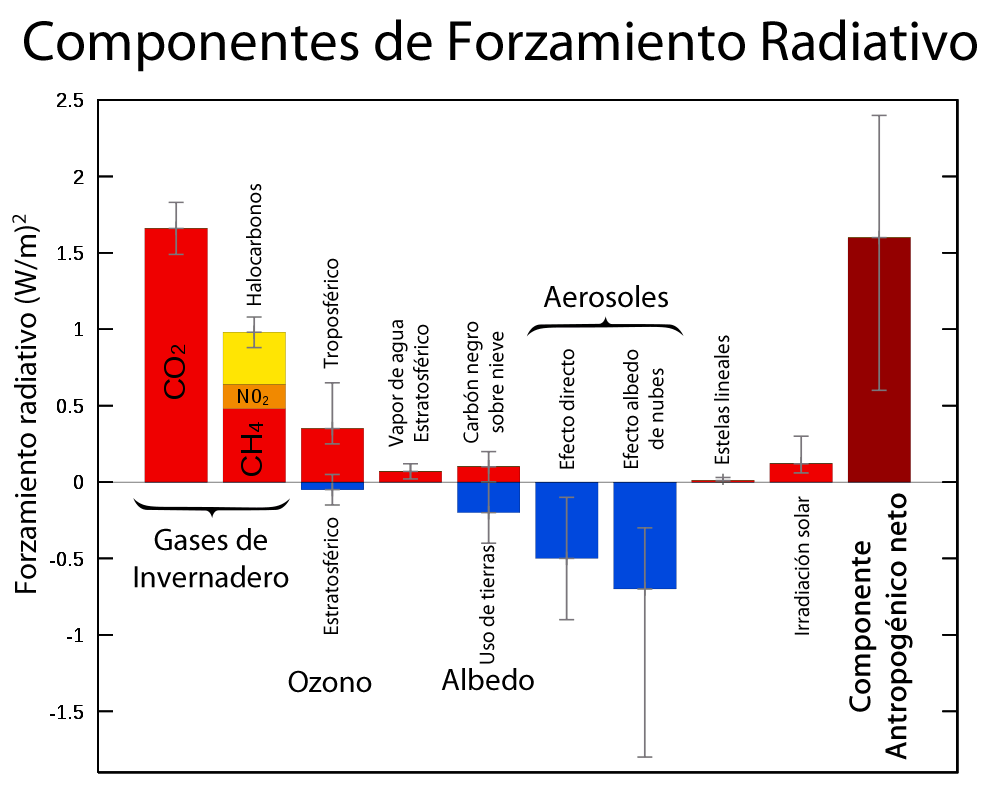
\includegraphics[width=\textwidth]{forzantes-radiativos.png}
\caption{Forzamiento radiativo de componentes atmosféricos.}
\label{CGWP}
\end{center}
\footnotesize{Fuente de Archivo: Radiative-forcings.es.svg. (2023, agosto 28). \textit{Wikimedia Commons}. Obtenida 03:30, Febrero 15, 2025 de \url{https://commons.wikimedia.org/w/index.php?title=File:Radiative-forcings.es.svg&oldid=796565394}.}

\end{minipage}
\end{figure}

Dependiendo del compuesto, su capacidad de absorción de radiación determina su potencial de calentamiento global, el cual se muestra en el \textbf{Cuadro~\ref{WGP}} (IPCC, \textup{4\textsuperscript{to}.} informe, 2007).


\begin{table}[htp]
\begin{minipage}{\linewidth}
\caption{Potencial de Calentamiento de varios compuestos}
\begin{center}
{\small \begin{tabular}{|l|l|r|r|r|}\hline
Nombre & Fórmula & Vida    & \multicolumn{2}{c}{Potencial Calentamiento Global} |\\
común  & química  & (años) &  100-años & 20 años \\\hline\hline
Dióxido de carbono & \ce{CO2} &       & 1   & 1 \\
Metano                    &  \ce{CH4} & 12 & 25 &72 \\
Oxido nitroso          &  \ce{N2O}  & 114& 289 &298\\  \hline
\multicolumn{5}{l}{Sustancias controladas por el Protocolo de Montreal}\\ \hline
CFC-11                  & \ce{CCl3F}    & 45   &  6,730 & 4,750 \\
CFC-12                 & \ce{CCl2F2}  & 100 &11,000 & 10,900 \\
CFC-115                & \ce{CClF2CF3}  &1,700 &5,310 & 7,370 \\
Halon-11301          & \ce{CBrF3}    & 65  & 8,480 & 7,140 \\
Tetracloruro de Carbono & \ce{CCl4} & 26 & 2,700 & 1,400 \\
Bromuro de metilo & \ce{CH3Br} & 0.7  &17 & 5 \\
HCFC-22               & \ce{CHClF2} & 12 & 5,160 & 1,810 \\
HCFC-123             & \ce{CHCl2CF3} & 1.3 & 273 & 77       \\ \hline
\multicolumn{5}{l}{Hidrofluorcarbonos}\\\hline
HFC-23                  &\ce{CHF3}  & 270 & 12,000 & 14,800 \\
HFC-32                  &\ce{CH2F3}  & 4.9 & 2,330 & 675 \\
HFC-125                & \ce{CHF2CF3} & 29 & 6,350 & 3,500 \\
HFC-134a              & \ce{CHFCF3} & 14 & 3,830 & 1,430 \\
HFC-236fa            & \ce{CF3CH2CF3} & 240 & 8,100 &9,810 \\ \hline
\multicolumn{5}{l}{Compuestos Perfluorinados}\\\hline
Hexafloruro de azufre & \ce{SF6}   & 3,200  & 16,300 &22,800 \\
Trifloruro de nitrógeno & \ce{NF3}  & 740     & 12,300 & 17,200 \\
PFC-14                        &\ce{CF4}   &50,000 & 5,210   &   7,390\\
PFC-116                        &\ce{C2F6}   &10,000 & 8,630 & 12,200\\ \hline
\end{tabular}}
\end{center}
\label{WGP}
\end{minipage}
\end{table}%


